\Opensolutionfile{ans}[ans/ansCD2D1-5]
\begin{dang}{Biện luận số giao điểm dựa vào đồ thị, bảng biến thiên}
\end{dang}
\paragraph{Các ví dụ}
\begin{vd}%Ví dụ 1.%[2D1Y5-4]
	\immini
	{
		Cho hàm số $y=f(x)$ liên tục trên $\mathbb{R}$ và có đồ thị như hình bên. Số nghiệm của phương trình $f(x)-1=0$ là
		\choice
		{$4$}
		{\True $3$}
		{$2$}
		{$1$}
	}
	{
		\begin{tikzpicture}[scale=.8]
		\draw[->] (-3,0)--(4,0);
		\draw[->] (0,-3)--(0,4);
		\draw[smooth,blue,line width=1] (-1.5, 1.83) .. controls (-1.1, 0.71) and (-0.72, 1.21) .. (-0.59, 1.39) 
		(-0.59, 1.39) .. controls (0.38, 2.7) and (1, 0) .. (1.28, -1.06)
		(1.28, -1.06) .. controls (2.08, -4.45) and (2.78, -1.05) .. (3.06, 1.31) ;
		\draw[dashed] (2,0)|-(0,-2.5) (-1,0)|-(0,1.14);
		\draw (-1,0) node[below]{$-1$}  (0,1.14) node[right]{$1$} 
		(2,0) node[below left]{$2$} (0,-2.5) node[left]{$\dfrac{-7}{2}$}  (0,0) node[below left]{$O$}  (4,0) node[below]{$x$}  (0,4) node[right]{$y$}   ;
		\foreach \y in {-2,-1,1,2}
		\draw[shift={(0,\y)}] (2pt,0)--(-2pt,0);
		\foreach \x in {-2,-1,1,2}
		\draw[shift={(\x,0)}] (0,2pt)--(0,-2pt);	
		\end{tikzpicture}
	}
	\loigiai{
		Số nghiệm của phương trình $f(x)-1=0$ là số giao điểm của đồ thị hàm số $y=f(x)$ và đường thẳng $y=1$.\\
		Dựa vào ĐTHS, suy ra số giao điểm là $3$.}
\end{vd}
\begin{vd}%Ví dụ 2.%[2D1Y5-3]
	\immini
	{
		Cho hàm số $y=f(x)$ xác định và liên tục trên $\mathbb{R}$, có bảng biến thiên.Số nghiệm của phương trình $2f(x)-1=0$ 
		\choice
		{$3$}
		{$2$}
		{$0$}
		{\True $1$} 
	}
	{
		\begin{tikzpicture}[scale=.7]
		\tkzTabInit[nocadre=false,lgt=1.5,espcl=3,deltacl=0.5]
		{$x$/1, $f’(x)$/1, $f(x)$/2.6}
		{$-\infty$,$1$,$3$,$+\infty$}
		\tkzTabLine{,+,z,-,z,+,}
		\draw ($(N13)!.2!(N12)$)node[below](A){$-\infty$} (N22)node[below](B){$0$} ($(N33)!.2!(N32)$)node[below](C){$-4$} (N42)node[below](D){$+\infty$};
		\draw[-stealth] (A)--(B);
		\draw[-stealth] (B)--(C);
		\draw[-stealth] (C)--(D);
		\end{tikzpicture}
	}	
	\loigiai{
		Ta có $2f(x)-1=0\Leftrightarrow f(x)=\dfrac{1}{2}$.
		\\ Dựa vào bảng biến thiên ta thấy phương trình có 1 nghiệm.}
\end{vd}
\begin{vd}%Ví dụ 3.%[2D1B5-4]
	\immini
	{
	Đồ thị sau đây là của hàm số $y=x^4-2x^2-3$. Với giá trị nào của $m$ thì phương trình $x^4-2x^2+m=0$ có ba nghiệm phân biệt?
	\choice
	{$m=-3$}
	{$m=-4$}
	{\True $m=0$}
	{$m=4$}
	}
	{
		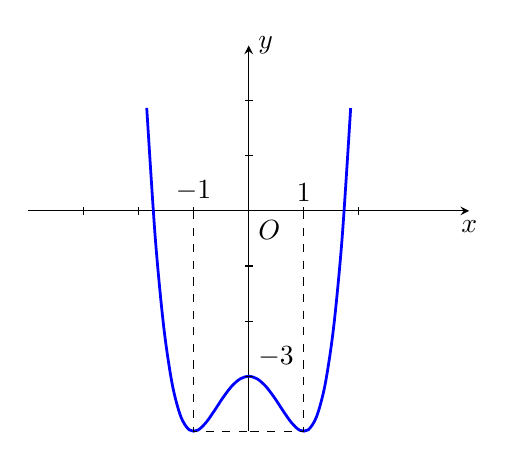
\begin{tikzpicture}[>=stealth,scale=.7]
		\draw[->] (-4,0) --(0,0) node[below
		right]{$O$} -- (4,0)
		node[below]{$x$};
		\draw[->](0,-4)--(0,3)
		node[right]{$y$};
		\draw[smooth,blue,line width=1]
		plot[domain=-1.85:1.85]
		(\x,{(\x)^(4)-2*(\x)^(2)-3});
		\draw[dashed] (-1,0)|-(0,-4) (1,0)|-(0,-4);
		\draw (-1,0) node[above]{$-1$} (1,0) node[above]{$1$} (0,-3) node[above right]{$-3$};
		\foreach \y in {-3,-2,-1,1,2}
		\draw[shift={(0,\y)}] (2pt,0)--(-2pt,0);
		\foreach \x in {-3,-2,-1,1,2}
		\draw[shift={(\x,0)}] (0,2pt)--(0,-2pt);
		\end{tikzpicture}
	}	
	\loigiai{
		Phương trình $x^4-2x^2+m=0$ 
		$ \Leftrightarrow x^4-2x^2-3=-m-3 $.\\
		Số nghiệm của phương trình $(1)$  là số giao điểm của đồ thị hàm số $y=x^4-2x^2-3$ và đường thẳng $y=-m-3$ có phương song song với trục hoành.\\
		Dựa vào đồ thị, phương trình có ba nghiệm phân biệt $\Leftrightarrow-m-3=-3\Leftrightarrow m=0 $. 
		\begin{center}
			\begin{tikzpicture}[>=stealth]
			\draw[->] (-4,0) --(0,0) node[below
			right]{$O$} -- (4,0)
			node[below]{$x$};
			\draw[->](0,-4)--(0,3)
			node[right]{$y$};
			\draw[smooth,blue,line width=1]
			plot[domain=-1.85:1.85]
			(\x,{(\x)^(4)-2*(\x)^(2)-3});
			\draw[dashed] (-1,0)|-(0,-4) (1,0)|-(0,-4);
			\draw (-1,0) node[above]{$-1$} (1,0) node[above]{$1$} (0,-3) node[above right]{$-3$};
			\foreach \y in {-3,-2,-1,1,2}
			\draw[shift={(0,\y)}] (2pt,0)--(-2pt,0);
			\foreach \x in {-3,-2,-1,1,2}
			\draw[shift={(\x,0)}] (0,2pt)--(0,-2pt);
			\draw (-3.5,-3)--(3.5,-3) ;
			\draw (3.5,-3) node [below]{$y=-m-3$};
			\end{tikzpicture}
		\end{center}
	}
\end{vd}
\begin{vd}%Ví dụ 4.%[2D1B5-4]
	Tìm các giá trị thực của tham số $m$ sao cho phương trình $-x^3-3x^2+2=m$ có ba nghiệm thực phân biệt?
	\choice
	{\True $m\in(-2;2)$}
	{$m\in\emptyset$}
	{$m\in(-2;1)$}
	{$m\in[-2;2]$}
	\loigiai{
		Xét hàm số $y=-x^3-3x^2+2$ trên $\mathbb{R}$, ta có $y'=-3x^2-6x=0\Leftrightarrow x=0\vee x=-2$.\\
		Bảng biến thiên: 
		\begin{center}
			\begin{tikzpicture}
			\tkzTabInit[nocadre=false,lgt=1.5,espcl=3,deltacl=0.5]
			{$x$/1, $f’(x)$/1, $f(x)$/2.9}
			{$-\infty$,$-2$,$0$,$+\infty$}
			\tkzTabLine{,-,z,+,z,-,}
			\draw (N12)node[below](A){$+\infty$} (N23)node[below](B){$-2$} (N32)node[below](C){$2$} (N43)node[below](D){$-\infty$};
			\draw[-stealth] (A)--(B);
			\draw[-stealth] (B)--(C);
			\draw[-stealth] (C)--(D);
			\end{tikzpicture}
		\end{center}
		Số nghiệm của phương trình $-x^3-3x^2+2=m$ là số giao điểm của đồ thị hàm số $y=-x^3-3x^2+2$ và đường thẳng $y=m$.\\
		Dựa vào bảng biến thiên ta thấy phương trình có $3$ nghiệm phân biệt $\Leftrightarrow-2<m<2$.}
\end{vd}
\begin{vd}%Ví dụ 5.%[2D1B5-4]
	Tìm tất cả các giá trị của tham số $m$ để đồ thị hàm số $y=x^4-2x^2+m$ cắt trục hoành tại đúng hai điểm.
	\choice
	{$m>3$}
	{$m<0$}
	{$m\leq 0$}
	{\True $m=1$ và $m<0$}
	\loigiai{
		Phương trình hoành độ giao điểm $x^4-2x^2+m=0\Leftrightarrow m=-x^4+2x^2$.\\
		Số nghiệm của phương trình là số giao điểm của đồ thị hàm số: $y=-x^4+2x^2$ và đường thẳng d: $y=m$.\\
		Khi đó dựa vào đồ thị ta thấy: $\hoac{&m=y_{CĐ}=1\\&m<y_{CT}=0}$ 
		\begin{center}
			\begin{tikzpicture}[>=stealth]
			\draw[->] (-4,0) --(0,0) node[below
			right]{$O$} -- (4,0)
			node[below]{$x$};
			\draw[->](0,-4)--(0,3)
			node[right]{$y$};
			\draw[smooth,blue,line width=1]
			plot[domain=-1.85:1.85]
			(\x,{-1*(\x)^(4)+2*(\x)^(2)});
			\draw (-1,0) node[below]{$-1$} (1,0) node[below]{$1$} ;
			\draw[dashed] (-1,0)|-(0,1) (1,0)|-(0,1);
			\foreach \y in {-3,-2,-1,1,2}
			\draw[shift={(0,\y)}] (2pt,0)--(-2pt,0);
			\foreach \x in {-3,-2,-1,1,2}
			\draw[shift={(\x,0)}] (0,2pt)--(0,-2pt);			
			\end{tikzpicture}
		\end{center}
	}
\end{vd}
\subsubsection{Câu hỏi trắc nghiệm}
\begin{ex}%Câu 1.%[2D1Y5-3]
	Cho hàm số $y=f(x)$ xác định, liên tục trên $\mathbb{R}$ và có bảng biến thiên sau: 
	\begin{center}
		\begin{tikzpicture}
		\tkzTabInit[nocadre=false,lgt=1.5,espcl=3,deltacl=0.5]
		{$x$/1, $f’(x)$/1, $f(x)$/2.6}
		{$-\infty$,$-1$,$0$,$1$,$+\infty$}
		\tkzTabLine{,-,z,+,z,-,0,+,}
		\draw (N12)node[below](A){$+\infty$} ($(N23)!.2!(N22)$)node[below](B){$-1$} (N32)node[below](C){$0$} ($(N43)!.2!(N42)$)node[below](D){$-1$} (N52)node[below](E){$+\infty$} ;
		\draw[-stealth] (A)--(B);
		\draw[-stealth] (B)--(C);
		\draw[-stealth] (C)--(D);
		\draw[-stealth] (D)--(E);
		\end{tikzpicture}
	\end{center}
	Số giao điểm của đồ thị hàm số $y=f(x)$ và trục hoành là
	\choice
	{$0$}
	{\True $3$}
	{$1$}
	{$2$}
	\loigiai{
		Theo bảng biến thiên ta thấy số giao điểm giữa đồ thị hàm số và trục hoành là $3$.}
\end{ex}
\begin{ex}%Câu 2.%[2D1B5-3]
	Cho hàm số $y=f(x)$ có bảng biến thiên như hình vẽ
	\begin{center}
		\begin{tikzpicture}
		\tkzTabInit[nocadre=false,lgt=1.5,espcl=3,deltacl=0.5]
		{$x$/1, $f’(x)$/1, $f(x)$/2.6}
		{$-\infty$,$-1$,$1$,$+\infty$}
		\tkzTabLine{,+,d,+,z,-,}
		\draw ($(N12)!.5!(N13)$)node[below](A){$2$} (N22)node[below left](B){$4$} ($(N22)!.8!(N23)$)node[below right](C){$-\infty$} ($(N32)!.2!(N33)$)node[below](D){$3$} ($(N42)!.7!(N43)$)node[below](E){$-1$} ;
		\draw[-stealth] (A)--(B);
		\draw[double] (N22)--(N23);
		\draw[-stealth] (C)--(D);
		\draw[-stealth] (D)--(E);
		\end{tikzpicture}
	\end{center}
	Số nghiệm của phương trình $f(x)-\dfrac{5}{2}=0$ là
	\choice
	{$0$}
	{$1$}
	{\True $3$}
	{$2$}
	\loigiai{
		Phương trình $f(x)-\dfrac{5}{3}=0\Leftrightarrow f(x)=\dfrac{5}{2}$
		Dựa vào bảng biến thiên ta thấy phương trình có 3 nghiệm.}
\end{ex}
\begin{ex}%Câu 3.%[2D1Y5-2]
	Cho hàm số $y=f(x)$ có bảng biến thiên như hình vẽ bên dưới. Số nghiệm của phương trình $f(x)+2=0$ là
	\begin{center}
		\begin{tikzpicture}
		\tkzTabInit[nocadre=false,lgt=1.5,espcl=3,deltacl=0.5]
		{$x$/1, $f’(x)$/1, $f(x)$/2.6}
		{$-\infty$,$-1$,$0$,$1$,$+\infty$}
		\tkzTabLine{,-,z,+,z,-,z,+,}
		\draw (N12)node[below](A){$+\infty$} ($(N23)!.2!(N22)$)node[below](B){$-4$} (N32)node[below](C){$-3$} ($(N43)!.2!(N42)$)node[below](D){$-4$} (N52)node[below](E){$+\infty$} ;
		\draw[-stealth] (A)--(B);
		\draw[-stealth] (B)--(C);
		\draw[-stealth] (C)--(D);
		\draw[-stealth] (D)--(E);
		\end{tikzpicture}
	\end{center}
	\choice
	{\True $2$}
	{$4$}
	{$3$}
	{$0$}
	\loigiai{
		Ta có	$f(x)+2=0\Leftrightarrow f(x)=-2$ nên phương trình này có hai nghiệm phân biệt.}
\end{ex}
\begin{ex}%Câu 4.%[2D1B5-3]
	Cho hàm số $f(x)=ax^4+bx^2+c$ có đồ thị như hình bên dưới. 
	\begin{center}
		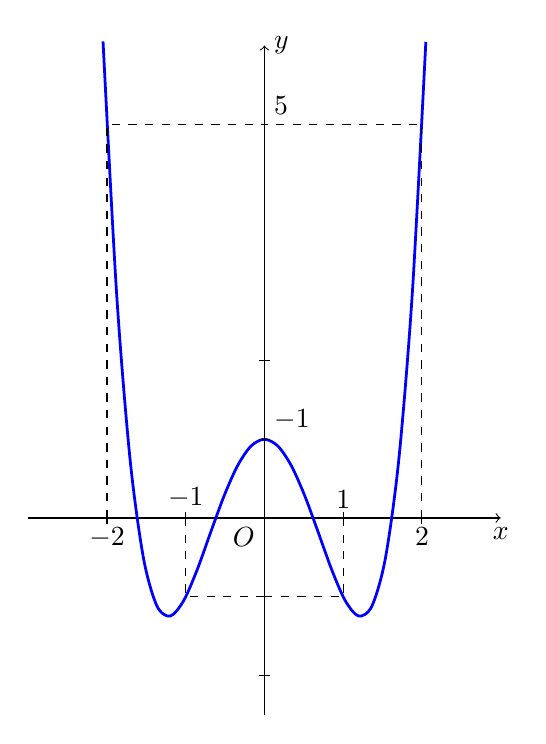
\begin{tikzpicture}%CÂU 4
		\draw[->] (-3,0)--(3,0);
		\draw[->] (0,-2.5)--(0,6);
		\draw  (0,0) node[below left]{$O$}  (3,0) node[below]{$x$}  (0,6) node[right]{$y$}   ;
		\draw[smooth,blue,line width=1]
		plot[domain=-2.05:2.05]
		(\x,{(\x)^(4)-3*(\x)^(2)+1});
		\draw[dashed] (-1,0)|-(0,-1) (1,0)|-(0,-1) (-2,0)|-(0,5) (2,0)|-(0,5) ;
		\draw (-1,0) node[above]{$-1$} (1,0) node[above]{$1$} (0,1) node[above right]{$-1$} (0,5) node[above right]{$5$} (2,0) node[below]{$2$} (-2,0) node[below]{$-2$};
		\foreach \y in {-2,-1,1,2}
		\draw[shift={(0,\y)}] (2pt,0)--(-2pt,0);
		\foreach \x in {-2,-1,1,2}
		\draw[shift={(\x,0)}] (0,2pt)--(0,-2pt);		
		\end{tikzpicture}
	\end{center}
	Tất cả các giá trị của tham số $m$ để phương trình $f(x)+2m=0$ có bốn nghiệm phân biệt là
	\choice
	{$-\dfrac{1}{2}<m<\dfrac{1}{2}$}
	{$-\dfrac{5}{4}<m<1$}
	{$-\dfrac{5}{8}<m<\dfrac{1}{2}$}
	{\True $-\dfrac{1}{2}<m<\dfrac{5}{8}$}
	\loigiai{
		Gọi $f(x)=ax^4+bx^2+c$ có đồ thị $(C)$.\\
		Vì $(C)$ qua các điểm $(0;1)$, $(1;-1)$, $(2;5)$ nên $f(x)=x^4-3x^2+1$.\\
		\[f'(x)=4x^3-6x=0\Leftrightarrow\hoac{&x=0\Rightarrow y_{CD}=1\\&x=\sqrt{\dfrac{3}{2}}\Rightarrow y_{CT}=-\dfrac{5}{4}\\&x=-\sqrt{\dfrac{3}{2}}\Rightarrow y_{CT}=-\dfrac{5}{4}.} \]
		Ta có $f(x)+2m=0\Leftrightarrow f(x)=-2m\ (1)$.\\
		Vì $(1)$ là phương trình hoành độ giao điểm của đồ thị $(C)$: $y=f(x)$ và đường thẳng $y=-2m$.\\
		Dựa vào đồ thị $(1)$ có bốn nghiệm phân biệt $\Leftrightarrow -\dfrac{5}{4} <-2m<1\Leftrightarrow-\dfrac{1}{2}<m<\dfrac{5}{8}$.}
\end{ex}
\begin{ex}%Câu 5.%[2D1B5-3]
	Cho hàm số $y=f(x)$ xác định và liên tục trên $\mathbb{R}$, có bảng biến thiên như sau:\\
	\begin{center}
		\begin{tikzpicture}
		\tkzTabInit[nocadre=false,lgt=1.5,espcl=3,deltacl=0.5]
		{$x$/1, $f’(x)$/1, $f(x)$/2.6}
		{$-\infty$,$-2$,$0$,$+\infty$}
		\tkzTabLine{,-,z,+,z,-,}
		\draw ($(N13)!.2!(N12)$)node[below](A){$-\infty$} (N22)node[below](B){$2$} ($(N33)!.2!(N32)$)node[below](C){$-2$} (N42)node[below](D){$+\infty$};
		\draw[-stealth] (A)--(B);
		\draw[-stealth] (B)--(C);
		\draw[-stealth] (C)--(D);
		\end{tikzpicture}
	\end{center}
	Tập hợp tất cả các giá trị của $m$ để phương trình $f(x)=m$ có đúng một nghiệm là
	\choice
	{\True $(-\infty;-2)\cup(2;+\infty)$}
	{$(-\infty;-2]\cup[2;+\infty)$}
	{$(-2;2)$}
	{$[-2;2]$}
	\loigiai{
		Dựa vào bảng biến thiên:\\
		Phương trình $f(x)=m$ có đúng một nghiệm\\
		$ \Leftrightarrow $ đồ thị hàm số $y=f(x)$ và đường thẳng $y=m$ có một giao điểm.\\
		$ \Leftrightarrow m\in(-\infty;-2)\cup(2;+\infty) $.}
\end{ex}
\begin{ex}%Câu 6.%[2D1B5-3]
	Cho hàm số $y=f(x)$ xác định trên tập $\mathscr{D}=\mathbb{R}\setminus\{-1\}$, liên tục trên mỗi khoảng xác định và có bảng biến thiên như sau: 
	\begin{center}
		
\begin{tikzpicture}
		\tkzTabInit[nocadre=false,lgt=1.5,espcl=2,deltacl=0.5]
		{$x$/.8, $f’(x)$/.8, $f(x)$/2}
		{$-\infty$,$-4$,$-1$,$2$,$+\infty$}
		\tkzTabLine{,+,z,-,d,-,z,+,}
		\tkzTabVar{-/$-\infty$ , +/$0$ , -D+/$-\infty$/$+\infty$ , -/$4$ , +/$+\infty$}
		\end{tikzpicture}
	\end{center}
	Tìm tập hợp tất cả các giá trị của $m$ sao cho phương trình $f(x)=m-1$ có hai nghiệm thực phân biệt. 
	\choice
	{\True $\hoac{&m<1\\&m>5}$}
	{$1<m<5$}
	{$m<1$}
	{$m>5$}
	\loigiai{
		Từ bảng biến thiên ta thấy phương trình $f(x)=m-1$ có hai nghiệm thực phân biệt  \[\Leftrightarrow \hoac{&m-1<0\\&m-1>4}\Leftrightarrow\hoac{&m<1\\&m>5.}\] }
\end{ex}
\begin{ex}%Câu 7.%[2D1Y5-3]
	Cho hàm số $y=f(x)=ax^4+bx^2+c$ có đồ thị như hình vẽ sau
	\begin{center}
		\begin{tikzpicture}%câu 7
		\draw[->] (-3,0)--(3,0);
		\draw[->] (0,-3)--(0,2.5);
		\draw  (0,0) node[below left]{$O$}  (3,0) node[below]{$x$}  (0,3) node[right]{$y$}   ;
		\draw[dashed] (-1,0)|-(0,-2.9) (1,0)|-(0,-2.9);
		\draw (-1,0) node[above]{$-1$} (1,0) node[above]{$1$} ( (0,-3) node[above right]{$-3$};
		\draw[smooth,blue] (-2.1, 2).. controls (-1.72, -0.48) and (-1.07, -5.76) .. (-0.47, -1.01)
		(-0.47, -1.01).. controls (-0.31, -0.04) and (0, 1.91) .. (0.46, -1.01)
		(0.46, -1.01).. controls (1.06, -5.99) and (1.81, 0.08) .. (2.1, 2)		
		; % Đường cong nối từ điểm (0,0) đến điểm (2,0) với 2 điểm kéo (0.5,1) và (1.5,-1)
		\foreach \y in {-2,-1,1,2}
		\draw[shift={(0,\y)}] (2pt,0)--(-2pt,0);
		\foreach \x in {-2,-1,1,2}
		\draw[shift={(\x,0)}] (0,2pt)--(0,-2pt);		
		\end{tikzpicture}
	\end{center}
	Số nghiệm của phương trình $f(x)-1=0$ là
	\choice
	{\True $3$}
	{$1$}
	{$4$}
	{$1$}
	\loigiai{
		Ta có $f(x)-1=0\Leftrightarrow f(x)=1$.\\
		Dựa vào đồ thị ta thấy đồ thị hàm số $y=f(x)$ và $y=1$ có $3$ giao điểm nên phương trình $f(x)-1=0$ có $3$ nghiệm phân biệt.}
\end{ex}
\begin{ex}%Câu 8.%[2D1Y5-3]
	Cho hàm số $y=f(x)$ liên tục và có đạo hàm trên tập xác định $\mathscr{D}=\mathbb{R}$. Biết rằng hàm số $y=f(x)$ có bảng biến thiên như sau:\\
	\begin{center}
		
\begin{tikzpicture}
		\tkzTabInit[nocadre=false,lgt=1.5,espcl=3,deltacl=0.5]
		{$x$/.8, $f’(x)$/.8, $f(x)$/2}
		{$-\infty$,$-1$,$1$,$+\infty$}
		\tkzTabLine{,-,z,+,z,-,}
		\tkzTabVar{+/$1$ , -/$\dfrac12$ , +/$\dfrac32$ , -/$1$}
		\end{tikzpicture}
	\end{center}
	Tìm tập hợp tất cả các giá trị của tham số thực $m$ để đồ thị hàm số $y=f(x)$ cắt đường thẳng $y=m$ tại hai điểm phân biệt. 
	\choice
	{$\left[\dfrac{1}{2};\dfrac{3}{2}\right]\setminus\{1\}$}
	{$\left(\dfrac{1}{2};\dfrac{3}{2}\right)$}
	{$\left[\dfrac{1}{2};\dfrac{3}{2}\right]$}
	{\True $\left(\dfrac{1}{2};\dfrac{3}{2}\right)\setminus\{1\}$}
	\loigiai{
		Dựa theo bảng biến thiên, yêu cầu bài toán $\Leftrightarrow m\in\left(\dfrac{1}{2};\dfrac{3}{2}\right)\setminus\{1\}$.}
\end{ex}
\begin{ex}%Câu 9.%[2D1B5-3]
	Tìm tất cả các giá trị của tham số thực $m$ để đồ thị hàm số $y=-x^2+4x+m-2$ không có điểm chung với trục hoành. 
	\choice
	{$m >-2$}
	{$m<2$}
	{$m>2$}
	{\True $m <-2$}
	\loigiai{
		Phương trình hoành độ giao điểm $-x^2+4x+m-2=0$.\\
		Yêu cầu bài toán khi vô nghiệm $\Leftrightarrow\Delta'<0\Leftrightarrow 4+m-2<0\Leftrightarrow m <-2$.}
\end{ex}
\begin{ex}%Câu 10.%[2D1B5-3]
	Cho hàm số $y=f(x)$ xác định trên $\mathbb{R}\setminus\{-1; 1\}$, liên tục trên từng khoảng xác định và có bảng biến thiên như sau: 
	\begin{center}
		
\begin{tikzpicture}
		\tkzTabInit[nocadre=false,lgt=1.5,espcl=2.5,deltacl=0.5]
		{$x$/.8, $f’(x)$/.8, $f(x)$/2}
		{$-\infty$,$-1$,$0$,$1$,$+\infty$}
		\tkzTabLine{,+,d,+,d,-,d,+,}
		\tkzTabVar{-/$3$ , +D-/$+\infty$/$-\infty$ , +/$2$ , -D-/$-\infty$/$-\infty$ , +/$-3$}
		\end{tikzpicture}
	\end{center}
	Tìm tất cả các giá trị thực của tham số $m$ sao cho phương trình $f(x)=3m$ có ba nghiệm phân biệt. 
	\choice
	{$-1<m<\dfrac{2}{3}$}
	{\True $m <-1$}
	{$m\leq-1$}
	{$m <-3$}
	\loigiai{
		Phương trình $f(x)=3m$ có ba nghiệm phân biệt $\Leftrightarrow 3m <-3\Leftrightarrow m <-1$.}
\end{ex}
\begin{ex}%Câu 11.%[2D1B5-3]
	Cho hàm số $y=f(x)$ xác định trên $\mathbb{R}\setminus\{1\}$, liên tục trên mỗi khoảng xác định và có bảng biến thiên như hình bên. Tìm tập hợp tất cả các giá trị thực của tham số $m$ sao cho phương trình $f(x)=m$ có ba nghiệm thực phân biệt. 
	\begin{center}
		
\begin{tikzpicture}
		\tkzTabInit[nocadre=false,lgt=1.5,espcl=3,deltacl=0.5]
		{$x$/.8, $f’(x)$/.8, $f(x)$/2}
		{$-\infty$,$-1$,$1$,$+\infty$}
		\tkzTabLine{,-,z,+,d,+,}
		\tkzTabVar{+/$1$ , -/$-\sqrt{2}$ , +D-/$+\infty$/$-\infty$ , +/$-1$}
		\end{tikzpicture}
	\end{center}
	\choice
	{$\left(-\sqrt{2};-1\right]$}
	{\True $\left(-\sqrt{2};-1\right)$}
	{$(-1;1]$}
	{$(-1;1)$}
	\loigiai{
		Số nghiệm của phương trình $f(x)=m$ là số giao điểm của đồ thị hàm số $y=f(x)$ và đường thẳng $y=m$.\\
		Dựa vào BBT để phương trình $f(x)=m$ có ba nghiệm thực phân biệt $\Leftrightarrow$ đường thẳng $y=m$ cắt đồ thị hàm số $y=f(x)$ tại 3 điểm phân biệt $\Leftrightarrow-\sqrt{2}<m <-1$.}
\end{ex}
\begin{ex}%Câu 12.%[2D1B5-3]
	Tìm tất cả các giá trị của $k$ để phương trình $4x^2\left(1-x^2\right)=1-k$ có bốn nghiệm thực phân biệt
	\choice
	{\True $0<k<1$}
	{$0<k<2$}
	{$k<3$}
	{$-1<k<1$}
	\loigiai{
		Xét hàm số $y=4x^2\left(1-x^2\right)=-4x^4+4x^2$.\\
		$y'=-16x^3+8x$.\\
		$y'=0\Leftrightarrow\hoac{&x=0\\&x=\pm\dfrac{1}{\sqrt{2}}.}$ \\
		$\lim\limits_{x\to+\infty} y=-\infty;\lim\limits_{x\to-\infty} y=-\infty$.\\
		BBT: 
		\begin{center}
			\begin{tikzpicture}
			\tkzTabInit[nocadre=false,lgt=1.5,espcl=3,deltacl=0.5]
			{$x$/1, $f’(x)$/1, $f(x)$/2.6}
			{$-\infty$,$-\dfrac{1}{\sqrt{2}}$,$0$,$\dfrac{1}{\sqrt{2}}$,$+\infty$}
			\tkzTabLine{,+,z,-,z,+,z,-,}
			\draw ($(N13)!.2!(N12)$)node[below](A){$-\infty$} (N22)node[below](B){$1$} ($(N33)!.2!(N32)$)node[below](C){$0$} (N42)node[below](D){$1$} ($(N53)!.2!(N52)$)node[below](E){$-\infty$} ;
			\draw[-stealth] (A)--(B);
			\draw[-stealth] (B)--(C);
			\draw[-stealth] (C)--(D);
			\draw[-stealth] (D)--(E);
			\end{tikzpicture}
		\end{center}
		Căn cứ vào BBT, để phương trình $4x^2\left(1-x^2\right)=1-k$ có bốn nghiệm thực phân biệt khi và chỉ khi $0<1-k<1\Leftrightarrow 0<k<1$.}
\end{ex}
\begin{ex}%Câu 13.%[2D1K5-3]
	Cho hàm số $y=f(x)$ có đồ thị như hình vẽ sau: 
	\begin{center}
		\begin{tikzpicture}%câu 13
		\draw[->] (-2,0)--(3,0);
		\draw[->] (0,-1)--(0,3);
		\draw  (0,0) node[below left]{$O$}  (3,0) node[below]{$x$}  (0,3) node[right]{$y$}   ;
		\draw[dashed] (0.9,0)|-(0,1.86);
		\draw (-0,2) node[above right]{$2$} (1,0) node[below]{$1$};
		\draw [smooth,blue,line width=1] (-0.7, 4) .. controls (-0.54, 2.08) and (-0.25, 0.44) .. (0.48, 1.51)
		(0.48, 1.51).. controls (0.76, 1.9) and (1.31, 2.74).. (1.6, -2)
		; 		
		% Đường cong nối từ điểm (0,0) đến điểm (2,0) với 2 điểm kéo (0.5,1) và (1.5,-1)
		%g(x) = -2.88(x - 1)³ + 4.77(x - 1)² - 0.89 (x - 1) + 1		
		\end{tikzpicture}
	\end{center}
	Số nghiệm của phương trình $2\cdot|f(x-1)|-3=0$ là 
	\choice
	{$1$}
	{\True $4$}
	{$3$}
	{$2$}
	\loigiai{
		Có phương trình $2\cdot|f(x-1)|-3=0\Leftrightarrow|f(x-1)|=\dfrac{3}{2}$.\\
		Ta chỉ cần tịnh tiến qua phải đồ thị đã cho 1 đơn vị rồi lật phần đồ thị dưới trục $Ox$ lên trên là được đồ thị hàm số $y=|f(x-1)|$. 
		\begin{center}
			\begin{tikzpicture}
			\draw[->] (-3,0)--(4,0);
			\draw[->] (0,-2.5)--(0,3);
			\draw  (0,0) node[above left]{$O$}  (3,0) node[below]{$x$}  (0,3) node[right]{$y$}   ;
			\draw[smooth,blue,line width=1]
			plot[domain=-.5:1.8]
			(\x,{-2.88*(\x)^(3)+4.77*(\x)^(2) -0.89*(\x)^(1) +1 });			
			\draw[smooth,red,line width=1]
			plot[domain=.5:2.8]
			(\x,{-2.88*(\x-1)^(3)+4.77*(\x-1)^(2) -0.89*(\x-1)^(1) +1 });
			\draw[smooth,gray,line width=1,dashed]
			plot[domain=2.6:2.9]
			(\x,{abs(-2.88*(\x-1)^(3)+4.77*(\x-1)^(2) -0.89*(\x-1)^(1) +1) });
			\node at (4.4, 3.08) {$y=\left|f(x-1)\right|$}; % Viết văn bản TEXT tại điểm (0,0) và đặt tên node là node1. Độ dài tối đa văn bản là 0.5\linewidth, văn bản canh giữa, xoay góc 30 độ,...
			\node at (-1.5, 3) {$y=f(x)$};
			\node at (4, -1) {$y=f(x-1)$};
			\draw[smooth,line width=1] (-2,1.5)--(3.5,1.5);
			\node at (4,1.5) {$y=\dfrac{3}{2}$};
			\foreach \y in {-2,-1,1,2}
			\draw[shift={(0,\y)}] (2pt,0)--(-2pt,0);
			\foreach \x in {-2,-1,1,2}
			\draw[shift={(\x,0)}] (0,2pt)--(0,-2pt);
			\end{tikzpicture}
		\end{center}
		Khi đó đồ thị hàm số $y=|f(x-1)|$ và đường thẳng $y=\dfrac{3}{2}$ cắt nhau tại 4 điểm. Vậy phương trình đã cho có 4 nghiệm.}
\end{ex}
\begin{ex}%Câu 14.%[2D1B5-3]
	Tìm tất cả các giá trị thực của tham số $m$ để phương trình $-x^4+2x^2+3+3m=0$ có $4$ nghiệm phân biệt. 
	\choice
	{$1<m<\dfrac{4}{3}$}
	{$-\dfrac{4}{3}\leq m\leq-1$}
	{$3<m<4$}
	{\True $-\dfrac{4}{3}<m <-1$}
	\loigiai{
		Ta có $-x^4+2x^2+3+3m=0\Leftrightarrow x^4-2x^2-3=3m(*)$.\\
		Xét hàm số $f(x)=x^4-2x^2-3$.\\
		Ta có $f'(x)=4x^3-4x; f'(x)=0\Leftrightarrow\hoac{&x=0\\&x=\pm 1.}$ \\
		Phương trình $(*)$ có $4$ nghiệm phân biệt $\Leftrightarrow f(1)<3m<f(0)\Leftrightarrow-4<3m <-3$ \\
		$ \Leftrightarrow-\dfrac{4}{3}<m <-1 $.}
\end{ex}
% \begin{ex}%Câu 15.%[2D1B5-3]
% 	Cho hàm số $y=ax^3+bx^2+cx+d$ có đồ thị trong hình bên. Hỏi phương trình $ax^3+bx^2+cx+d=0$ có bao nhiêu nghiệm?\\
% 	{\color{red} HINH O DAY}\\
% 	\choice
% 	{Phương trình không có nghiệm}
% 	{Phương trình có đúng một nghiệm}
% 	{Phương trình có đúng hai nghiệm}
% 	{\True Phương trình có đúng ba nghiệm}
% 	\loigiai{
% 		Quan sát đồ thị ta thấy đồ thị hàm số cắt trục $Ox$ tại $3$ điểm phân biệt. \\
% 		Vậy phương trình $ax^3+bx^2+cx+d=0$ có $3$ nghiệm phân biệt.}
% \end{ex}
\begin{ex}%Câu 16.%[2D1K5-3]
	Tìm $m$ để phương trình sau có nghiệm: $\left(\sqrt{4-x}+\sqrt{4+x}\right)^3-6\sqrt{16-x^2}+2m+1=0$ 
	\choice
	{$m\in\mathbb{R}$}
	{$m>\dfrac{-1-16\sqrt{2}}{2}$}
	{\True $-\dfrac{41}{2}\leq m\leq\dfrac{-1-16\sqrt{2}}{2}$}
	{$m <-\dfrac{41}{2}$}
	\loigiai{
		Điều kiện: $x\in[-4;4]$.\\
		Đặt t= $\sqrt{4-x}+\sqrt{4+x}$.\\
		Ta có: $t'=-\dfrac{1}{2\sqrt{4-x}}+\dfrac{1}{2\sqrt{4+x}}=0\Rightarrow x=0$.\\
		Vậy khi $x\in[-4;4]$ thì $t\in\left[2\sqrt{2};4\right]$.\\
		Bài toán trở thành tìm $m$ để phương trình:\\
		$t^3-3\left(t^2-8\right)+2m+1=0$ có nghiệm trong đoạn $\left[2\sqrt{2};4\right]$ \\
		$ \Leftrightarrow t^3-3t^2+2m+25=0 $ có nghiệm trong đoạn $\left[2\sqrt{2};4\right]$.\\
		Xét hàm số $y=t^3-3t^2+25\Rightarrow y'=3t^2-6t=0\Rightarrow\hoac{&t=0\\&t=2}(L)$.\\
		Ta có $y(2\sqrt{2})=1+16\sqrt{2};\ y(4)=41$.\\
		Yêu cầu bài toán $(*)\Leftrightarrow 1+16\sqrt{2}\leq-2m\leq 41\Leftrightarrow-\dfrac{41}{2}\leq m\leq\dfrac{-1-16\sqrt{2}}{2}$.}
\end{ex}
\begin{ex}%Câu 17.%[2D1K5-3]
	Tìm tất cả các giá trị thực của tham số $m$ để phương trình $x^4-3x^2-m-1=0$ có hai nghiệm phân biệt. 
	\choice
	{\True $m >-1$ hoặc $m=-\dfrac{13}{4}$}
	{$m >-1$}
	{$m\geq-1$ hoặc $m=-\dfrac{13}{4}$}
	{$m\geq-1$}
	\loigiai{
		Xét hàm số $f(x)=x^4-3x^2$ có $f'(x)=4x^3-6x=0\Leftrightarrow\hoac{&x=0\\&x=\pm\dfrac{\sqrt{6}}{2}.}$ \\
		Tính giá trị $f(0)=0$, $f\left(\pm\dfrac{\sqrt{6}}{2}\right)=-\dfrac{9}{4}$ suy ra đồ thị $(C)$ của hàm số $y=f(x)$. 
		\begin{center}
			\begin{tikzpicture}%CÂU 17
			\draw[->] (-3,0)--(3,0);
			\draw[->] (0,-2.5)--(0,2);
			\draw  (0,0) node[above left]{$O$}  (3,0) node[below]{$x$}  (0,2) node[right]{$y$};
			\clip (-3+0.1,-2.5+0.1) rectangle (3-0.1,2-0.1);
			\draw[smooth]	plot[domain=-2.01:2.01]
			(\x,{(\x)^(4)-3*(\x)^(2)});
			\foreach \y in {-2,-1,1,2,3,4}
			\draw[shift={(0,\y)}] (2pt,0)--(-2pt,0);
			\foreach \x in {-2,-1,1,2}
			\draw[shift={(\x,0)}] (0,2pt)--(0,-2pt);			
			\end{tikzpicture}
		\end{center}
		Để phương trình $f(x)=m+1$ có hai nghiệm phân biệt $\Leftrightarrow\hoac{&m+1>0\\&m+1=-\dfrac{9}{4}}\Leftrightarrow\hoac{&m >-1\\&m=-\dfrac{13}{4}}$.}
\end{ex}
\begin{ex}%Câu 18.%[2D1K5-3]
	Cho hàm số $y=f(x)$ có đồ thị như hình vẽ. Với các giá trị nào của tham số $m$ thì phương trình $f(|x|)=3m+1$ có $4$ nghiệm phân biệt. 
	\begin{center}
		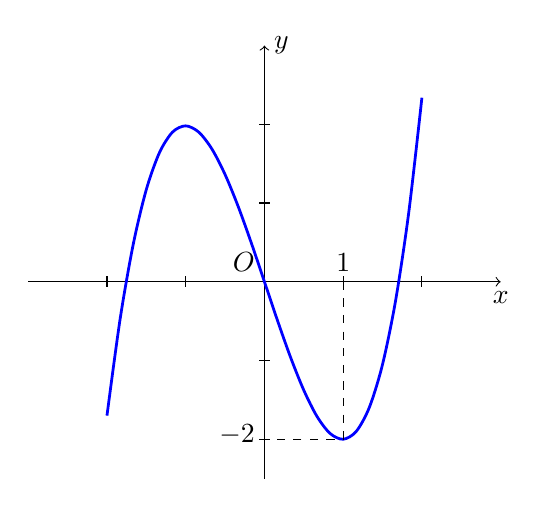
\begin{tikzpicture}%CÂU 18 PHẦN ĐỀ
		\draw[->] (-3,0)--(3,0);
		\draw[->] (0,-2.5)--(0,3);
		\draw  (0,0) node[above left]{$O$}  (3,0) node[below]{$x$}  (0,3) node[right]{$y$}   ;
		\draw[smooth,blue,line width=1]
		plot[domain=-2:2]
		(\x,{0.03*(\x)^(4)+1*(\x)^(3) -0.04*(\x)^(2)-2.99*(\x)^(1) });
		\draw[dashed] (1,0)|-(0,-2);
		\draw (-0,-2.2) node[above left]{$-2$} (1,0) node[above]{$1$};
		\foreach \y in {-2,-1,1,2}
		\draw[shift={(0,\y)}] (2pt,0)--(-2pt,0);
		\foreach \x in {-2,-1,1,2}
		\draw[shift={(\x,0)}] (0,2pt)--(0,-2pt);		
		%f(x) = 0.03x⁴ + 1x³ - 0.04x² - 2.99x
		\end{tikzpicture}
	\end{center}
	\choice
	{$m <-1$}
	{\True $-1<m <-\dfrac{1}{3}$}
	{$1<m<2$}
	{$m<2$}
	\loigiai{
		\begin{center}
			\begin{tikzpicture}%CÂU 18 PHẦN LỜI GIẢI
			\draw[->] (-3,0)--(3,0);
			\draw[->] (0,-2.5)--(0,3);
			\draw  (0,0) node[above left]{$O$}  (3,0) node[below]{$x$}  (0,3) node[right]{$y$}   ;
			\draw[smooth,blue,line width=1]
			plot[domain=0:2]
			(\x,{0.03*(\x)^(4)+1*(\x)^(3) -0.04*(\x)^(2)-2.99*(\x)^(1) });
			\draw[smooth,blue,line width=1,dashed]
			plot[domain=-2:0]
			(\x,{0.03*(\x)^(4)-1*(\x)^(3) -0.04*(\x)^(2)+2.99*(\x)^(1) });
			\draw[dashed] (1,0)|-(0,-2);
			\draw (-0,-2.2) node[above left]{$-2$} (1,0) node[above]{$1$};
			\draw (-2.5,-1.5)--(2.5,-1.5) ;
			\draw (3,-1)node[below]{$y=3m+1$};
			\foreach \y in {-2,-1,1,2}
			\draw[shift={(0,\y)}] (2pt,0)--(-2pt,0);
			\foreach \x in {-2,-1,1,2}
			\draw[shift={(\x,0)}] (0,2pt)--(0,-2pt);			
			%f(x) = 0.03x⁴ + 1x³ - 0.04x² - 2.99x
			\end{tikzpicture}
		\end{center}
		Từ đồ thị $y=f(x)$ ta suy được đồ thị $y=f(|x|)$ như hình bên.\\
		Số nghiệm của phương trình $f(|x|)=3m+1$ là số giao điểm của đồ thị $y=f(|x|)$ và đường thẳng $y=3m+1$.\\
		Do đó phương trình $f(|x|)=3m+1$ có $4$ nghiệm phân biệt khi:\\
		\[-2<3m+1<0\Leftrightarrow -1<m <-\dfrac{1}{3}\]	}
\end{ex}
\begin{ex}%Câu 19.%[2D1K5-3]
	Tập hợp tất cả các giá trị của tham số thực $m$ sao cho phương trình $\dfrac{\left||x|-2\right|}{|x|+1}=m$ có đúng $2$ nghiệm phân biệt là
	\choice
	{$[1;2]\cup\{0\}$}
	{\True $[1;2)\cup\{0\}$}
	{$[0;2)$}
	{$[1;2)$}
	\loigiai{
		Ta có đồ thị hàm số $y=\dfrac{\left||x|-2\right|}{|x|+1}$ là
\begin{center}
		\begin{tikzpicture}
	\draw[->] (-4,0)--(4,0);
	\draw[->] (0,-2.5)--(0,4);
	\draw  (0,0) node[below left]{$O$}  (4,0) node[below]{$x$}  (0,4) node[right]{$y$}   ;
	\draw[smooth,blue,line width=1]
	plot[domain=-4:4]
	(\x,{abs(abs(\x)-2)/(abs(\x)+1)});
	%f(x) = -0.5x³ + 1.5x
	\foreach \y in {-2,-1,1,2,3}
	\draw[shift={(0,\y)}] (2pt,0)--(-2pt,0);
	\foreach \x in {-2,-1,1,2,3}
	\draw[shift={(\x,0)}] (0,2pt)--(0,-2pt);	
	\draw (-1,0) node[below]{$-1$} (-2,0) node[below]{$-2$} (-3,0) node[below]{$-3$}
	(1,0) node[below]{$1$} (2,0) node[below]{$2$} (3,0) node[below]{$3$}	
	; 
	\draw[red,smooth] (-4,1)--(4,1);	
	\end{tikzpicture}
\end{center}
		Dựa vào đồ thị suy ra phương trình $\dfrac{\left||x|-2\right|}{|x|+1}=m$ có đúng $2$ nghiệm phân biệt $\Leftrightarrow m\in[1;2)\cup\{0\}$.}
\end{ex}
\begin{ex}%Câu 20.%[2D1K5-3]
	Cho hàm số $y=f(x)$ liên tục trên $\mathbb{R}$ và có đồ thị như hình vẽ. 
	\begin{center}
		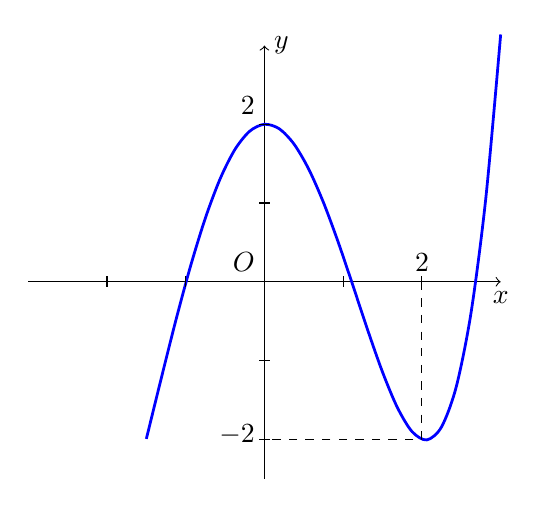
\begin{tikzpicture}%CÂU 20 PHẦN ĐỀ
		\draw[->] (-3,0)--(3,0);
		\draw[->] (0,-2.5)--(0,3);
		\draw  (0,0) node[above left]{$O$}  (3,0) node[below]{$x$}  (0,3) node[right]{$y$}   ;
		\draw[smooth,blue,line width=1]
		plot[domain=-1.5:3]
		(\x,{0.21*(\x)^(4)+0.09*(\x)^(3) -2.06*(\x)^(2)+0.08*(\x)^(1) +2 });		
		\draw[dashed] (2,0)|-(0,-2);
		\draw (-0,-2.2) node[above left]{$-2$} (2,0) node[above]{$2$} (0,2) node[above left]{$2$} ;
		\foreach \y in {-2,-1,1,2}
		\draw[shift={(0,\y)}] (2pt,0)--(-2pt,0);
		\foreach \x in {-2,-1,1,2}
		\draw[shift={(\x,0)}] (0,2pt)--(0,-2pt);		
		\end{tikzpicture}
	\end{center}
	Gọi $m$ là số nghiệm thực của phương trình $f\left(f(x)\right)=1$. Khẳng định nào sau đây là đúng?
	\choice
	{$m=6$}
	{\True $m=7$}
	{$m=5$}
	{$m=9$}
	\loigiai{
		Ta có $f\left(f(x)\right)=1\Leftrightarrow\hoac{&f(x)=a\ (-1<a<0)\ (1)\\&f(x)=b\ (0<b<1)\ (2)\\&f(x)=c\ (2<c<3)\ (3).}$ \\
		Ta thấy phương trình $(1)$ có $3$ nghiệm phân biệt; phương trình $(2)$ có $3$ nghiệm phân biệt; phương trình $(3)$ có đúng $1$ nghiệm và các nghiệm này không trùng nhau.\\
		Vậy phương trình $f\left(f(x)\right)=1$ có tất cả $7$ nghiệm.}
\end{ex}
\begin{ex}%Câu 21.%[2D1K5-3]
	Tìm m để đồ thị của hàm số $y=x^3-3x^2+4$ và đường thẳng $y=mx+m$ cắt nhau tại 3 điểm phân biệt $A(-1; 0)$, B, C sao cho tam giác $OBC$ có diện tích bằng 8. 
	\choice
	{$m=3$}
	{$m=1$}
	{\True $m=4$}
	{$m=2$}
	\loigiai{
		+ Để đồ thị của hàm số $y=x^3-3x^2+4$ cắt đường thẳng d: $y=mx+m$ tại 3 điểm phân biệt là phương trình sau có 3 nghiệm phân biệt:\\
		\allowdisplaybreaks
		\[\begin{aligned}
		x^3-3x^2+4=mx+m&\Leftrightarrow  (x+1)(x^2-4x+4-m)=0\\&\Leftrightarrow \hoac{&x=-1\\&x^2-4x+4-m=0 (*)}\\&\Rightarrow\heva{&m\neq 9\\&m>0 } \end{aligned}\]
		\\
		+ Khi đó $B(x_1; mx_1+m), B(x_2; mx_2+m)$, $x_1, x_2$ là 2 nghiệm của $(*)$.\\
		Ta có: $S_{OBC}=\dfrac{1}{2}BC\cdot d[O,BC]=8\Leftrightarrow\dfrac{1}{2}\sqrt{\left(m^2+1\right)\left[(x_1+x_2)^2-4x_1x_2\right]}\cdot\dfrac{|m|}{\sqrt{m^2+1}}=8$ \\
		$ \Leftrightarrow\sqrt{16-4(4-m)}\cdot|m|=16\Leftrightarrow m^3=64\Leftrightarrow m=4 $.\\
		Vậy $m = 4$.}
\end{ex}
\begin{ex}%Câu 22.%[2D1G5-3]
	Cho hàm số $f(x)=x^3+ax^2+bx+c$. Nếu phương trình $f(x)=0$ có ba nghiệm phân biệt thì phương trình $2f(x)\cdot f''(x)=[f'(x)]^2$ có nhiều nhất bao nhiêu nghiệm?
	\choice
	{$3$ nghiệm}
	{$1$ nghiệm}
	{\True $2$ nghiệm}
	{$4$ nghiệm}
	\loigiai{
		Xét hàm số $g(x)=2f(x)\cdot f''(x)-[f'(x)]^2$. \\
		Ta có: $f'''(x)=6$.\\
		Do $g'(x)=2f'(x)\cdot f''(x)+2f(x)\cdot f'''(x)-2f'(x)\cdot f''(x)=12f(x)$ nên $g'(x)=0$ có ba nghiệm phân biệt.\\
		Dễ thấy $g(x)=0$ là một phương trình bậc bốn.\\
		Gọi $x_1, x_2, x_3$ là nghiệm của phương trình $f(x)=0$. \\
		Do đó $x_1, x_2, x_3$ không là nghiệm của phương trình $f'(x)=0$.\\
		Ta có: $g(x_1)=-[f'(x_1)]^2<0, g(x_2)=-[f'(x_2)]^2<0, g(x_3)=-[f'(x_3)]^2<0$.\\
		Mà hệ số của $x^4$ trong phương trình $g(x)=0$ là $3>0$.\\
		Do đó phương trình $g(x)=0$ có nhiều nhất là $2$ nghiệm.\\
		Ví dụ $f(x)=x^3-x$ thỏa mãn.}
\end{ex}
\begin{ex}%Câu 23.%[2D1K5-3]
	Cho hàm số $y=x^3-3x^2$ có đồ thị $(C)$ như hình vẽ. Dựa vào đồ thị $(C)$, tìm $m$ để phương trình $\left(\sqrt{2-x}+\sqrt{x+1}\right)^3-6\sqrt{2+x-x^2}=m$ có nghiệm thực. 
	\begin{center}
		\begin{tikzpicture}%CÂU 23 PHẦN ĐỀ
		\draw[->] (-3,0)--(3.8,0);
		\draw[->] (0,-4.4)--(0,3);
		\draw  (0,0) node[above left]{$O$}  (3.8,0) node[below]{$x$}  (0,3) node[right]{$y$}   ;
		\draw[smooth,blue,line width=1]
		plot[domain=-1.1:3.15]
		(\x,{0.96*(\x)^(3) -2.79*(\x)^(2)-0.258*(\x)^(1) });		
		\draw[dashed] (2,0)|-(0,-4);
		\draw (-0,-4) node[above left]{$-4$} (2,0) node[above]{$2$} (0,-2) node[above left]{$-2$};				
		%f(x) = 0.96x³ - 2.79x² - 0.25x
		\foreach \y in {-4,-3,-2,-1,1,2}
		\draw[shift={(0,\y)}] (2pt,0)--(-2pt,0);
		\foreach \x in {-2,-1,1,2}
		\draw[shift={(\x,0)}] (0,2pt)--(0,-2pt);		
		\end{tikzpicture}
	\end{center}
	\choice
	{$-9\leq m\leq 6\sqrt{6}-9$}
	{$3\sqrt{3}-9\leq m\leq 6\sqrt{6}-9$}
	{$5\leq m\leq 3\sqrt{6}-9$}
	{\True $5\leq m\leq 6\sqrt{6}-9$}
	\loigiai{
		Ta có\\
		$\left(\sqrt{2-x}+\sqrt{x+1}\right)^3-6\sqrt{2+x-x^2}=m\Leftrightarrow\left(\sqrt{2-x}+\sqrt{x+1}\right)^3-3\left(\sqrt{2-x}+\sqrt{x+1}\right)^2=m-9$.\\
		Điều kiện: $-1\leq x\leq 2$.\\
		Đặt $t=\sqrt{2-x}+\sqrt{x+1}\ \left(\sqrt{3}\leq t\leq\sqrt{6}\right)$.\\
		Ta được phương trình $t^3-3t^2=m-9$.\\
		Phương trình $\left(\sqrt{2-x}+\sqrt{x+1}\right)^3-6\sqrt{2+x-x^2}=m$ có nghiệm thực khi phương trình $t^3-3t^2=m-9$ có nghiệm $t\in\left[\sqrt{3};\sqrt{6}\right]$.\\
		Xét hàm số $f(t)=t^3-3t^2$.\\
		Dựa vào đồ thị suy ra phương trình $t^3-3t^2=m-9$ có nghiệm $t\in\left[\sqrt{3};\sqrt{6}\right]$ khi
		\[-4\leq m-9\leq f(\sqrt{6})\Leftrightarrow 5\leq m\leq 6\sqrt{6}-9.\]
		}
\end{ex}
\begin{ex}%Câu 24.%[2D1K5-3]
	Cho hàm số $y=4x^3-6x^2+1$ có đồ thị như hình vẽ.\\
	\begin{center}
		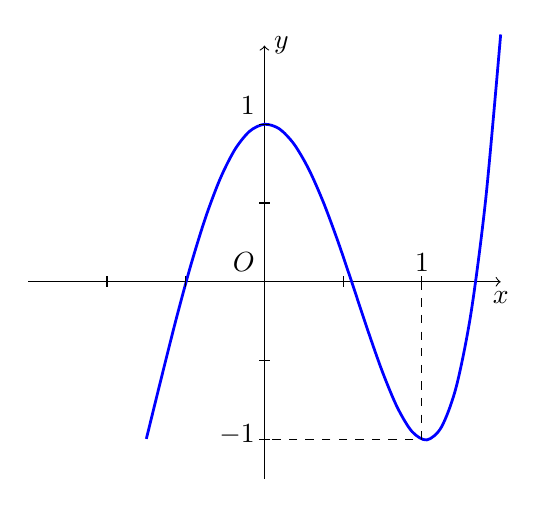
\begin{tikzpicture}%CÂU 20 PHẦN ĐỀ
		\draw[->] (-3,0)--(3,0);
		\draw[->] (0,-2.5)--(0,3);
		\draw  (0,0) node[above left]{$O$}  (3,0) node[below]{$x$}  (0,3) node[right]{$y$}   ;
		\draw[smooth,blue,line width=1]
		plot[domain=-1.5:3]
		(\x,{0.21*(\x)^(4)+0.09*(\x)^(3) -2.06*(\x)^(2)+0.08*(\x)^(1) +2 });		
		\draw[dashed] (2,0)|-(0,-2);
		\draw (-0,-2.2) node[above left]{$-1$} (2,0) node[above]{$1$} (0,2) node[above left]{$1$} ;
		\foreach \y in {-2,-1,1,2}
		\draw[shift={(0,\y)}] (2pt,0)--(-2pt,0);
		\foreach \x in {-2,-1,1,2}
		\draw[shift={(\x,0)}] (0,2pt)--(0,-2pt);	
		\end{tikzpicture}
	\end{center}
	Khi đó phương trình $4\left(4x^3-6x^2+1\right)^3-6\left(4x^3-6x^2+1\right)^2+1=0$ có bao nhiêu nghiệm thực?
	\choice
	{$3$}
	{$6$}
	{\True $7$}
	{$9$}
	\loigiai{
		Đặt $t=4x^3-6x^2+1\Rightarrow t\in \mathbb{R}$.\\
		Ta có: $4\left(4x^3-6x^2+1\right)^3-6\left(4x^3-6x^2+1\right)^2+1=0\Leftrightarrow 4t^3-6t^2+1=0$.\\
		Dựa vào đồ thị ta thấy phương trình có $3$ nghiệm $t_1,t_2,t_3$ trong đó $-1<t_1<0,\ 0<t_2<1,\ 1<t_3<2$.\\
		Khi $4x^3-6x^2+1=t_1$ dựa vào đồ thị ta thấy phương trình này có $3$ nghiệm.\\
		Khi $4x^3-6x^2+1=t_2$ dựa vào đồ thị ta thấy phương trình này có $3$ nghiệm.\\
		Khi $4x^3-6x^2+1=t_3$ dựa vào đồ thị ta thấy phương trình này có $1$ nghiệm.\\
		Vậy phương trình ban đầu có đúng $7$ nghiệm.}
\end{ex}
\begin{ex}%Câu 25.%[2D1K5-3]
	Cho hàm số $y=f(x)$ liên tục trên $\mathbb{R}$ và có bảng biến thiên như hình vẽ. 
	\begin{center}
		
\begin{tikzpicture}
			\tkzTabInit[nocadre=false,lgt=1.5,espcl=3,deltacl=0.5]
			{$x$/.8, $f’(x)$/.8, $f(x)$/2}
			{$-\infty$,$-1$,$1$,$+\infty$}
			\tkzTabLine{,-,z,+,z,-,}
			\tkzTabVar{+/$1$ , -/$\dfrac12$ , +/$\dfrac32$ , -/$1$}
			\end{tikzpicture}
	\end{center}
	Tìm tât cả các giá trị của tham số $m$ sao cho phương trình $\left|f(x-2018)+2\right|=m$ có 4 nghiệm thực phân biệt?
	\choice
	{$-3<m<1$}
	{$0<m<1$}
	{Không có giá trị của $m$}
	{\True $1<m<3$}
	\loigiai{
		Cách 1.
		Tịnh tiến $f(x)$ sang phải 2018 đơn vị sau đó lên trên 2 đơn vị ta được đồ thị hàm số $y=f(x-2018)+2$.\\
		Từ đó suy ra bảng biến thiên của hàm số $y=\left|f(x-2018)+2\right|$ 
		\begin{center}
			% \begin{tikzpicture}
			% \tkzTabInit[nocadre=false,lgt=1.5,espcl=3,deltacl=0.5]
			% {$x$/.8, $f’(x)$/.8, $f(x)$/2}
			% {$-\infty$,$-1$,$1$,$+\infty$}
			% \tkzTabLine{,-,z,+,z,-,}
			% \tkzTabVar{+/$1$ , -/$\dfrac12$ , +/$\dfrac32$ , -/$1$}
			% \end{tikzpicture}
		\end{center}
		Dựa vào bảng biến thiên thì giá trị $m$ cần tìm là $1<m<3$.\\
		Cách 2.
		Đặt $g(x)=f(x-2018)+2$, $g'(x)=f'(x-2018)$, $g'(x)=0\Leftrightarrow\hoac{&x-2018=0\\&x-2018=2}\Leftrightarrow\hoac{&x=2018\\&x=2020.}$ \\
		Bảng biến thiên
		\begin{center}
			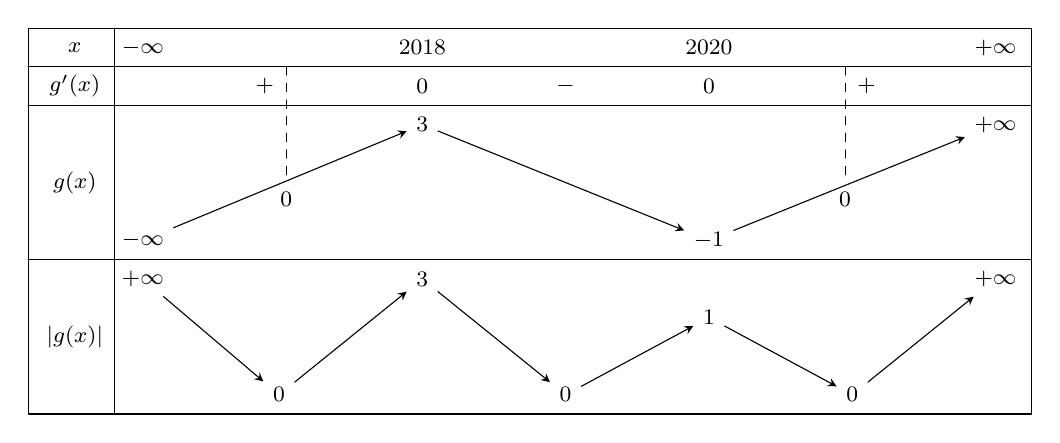
\begin{tikzpicture}[scale=0.7, font=\footnotesize, line join=round, line cap=round,>=stealth,yscale=.7,xscale=1.3]
			\def\cot{13} % số nhãn chiều dài
			\def\hang{9} % số nhãn chiều cao
			\draw[shift={(-.5,.5)}] 
			(0,0) rectangle +(\cot+1,-\hang-1)
			(0,-1)--+(0:\cot+1) 
			(0,-2)--+(0:\cot+1) 
			(0,-6)--+(0:\cot+1)
			(1.2,0)--+(-90:\hang+1);
			\path 
			(0.15,0) node{$x$} 
			(1.1,0) node{$-\infty$}
			(5,0) node{$2018$}
			(9,0) node{$2020$}												 	
			(13,0) node{$+\infty$}	
			(0.15,-1) node{$g'(x)$}
			(2.8,-1) node{$+$}
			(5,-1) node{$0$}
			(7,-1) node{$-$}
			(9,-1) node{$0$}
			(11.2,-1) node{$+$}
			(0.15,-3.5) node{$g(x)$}
			(1.1,-5) node (avc) {$-\infty$}
			(5,-2) node (ba) {$3$}
			(9,-5) node (mott) {$-1$}
			(13,-2) node (dvc1) {$+\infty$}											 	
			(0.15,-7.5) node{$|g(x)|$}
			(1.1,-6) node (dvcL) {$+\infty$}												
			(5,-6) node (CD1) {$3$}
			(3,-9) node (ko1) {$0$}
			(7,-9) node (ko2) {$0$}
			(11,-9) node (ko3) {$0$}
			(9,-7) node (CD2) {$1$}
			(13,-6) node (dvcR) {$+\infty$}
			;
			\draw[dashed] (3.1,-0.5)--(3.1,-3.5)node[below]{$0$};
			\draw[dashed] (10.9,-0.5)--(10.9,-3.5)node[below]{$0$};
			\draw[->] (avc)--(ba);
			\draw[->] (ba)--(mott);
			\draw[->] (mott)--(dvc1);
			\draw[->] (dvcL)--(ko1);
			\draw[->] (ko1)--(CD1);
			\draw[->] (CD1)--(ko2);
			\draw[->] (ko2)--(CD2);
			\draw[->] (CD2)--(ko3);
			\draw[->] (ko3)--(dvcR);
			\end{tikzpicture}
		\end{center}
		Dựa vào bảng biến thiên thì giá trị $m$ cần tìm là $1<m<3$.}
\end{ex}
\Closesolutionfile{ans}